\documentclass[11pt]{article}

\usepackage{amsmath,amssymb,amsfonts}
\usepackage{graphicx}
\usepackage{booktabs}
\usepackage{algorithm}
\usepackage{algpseudocode}
\usepackage{geometry}
\usepackage{hyperref}
\usepackage{float}

\geometry{margin=1in}

\title{
Explainable Regime Investing: Parametric vs.\ Non-Parametric Regime Detection
}

\author{Amine Boukardagha }
\date{Columbia University}

\begin{document}
\maketitle

\begin{abstract}
We study explainable, regime-aware portfolio construction at daily frequency in a diversified cross-asset universe.
Our central contribution is a practical \textbf{parametric regime detection} framework designed for production:
a strictly causal Gaussian Hidden Markov Model (HMM) with \textbf{predictive model-order selection} and
\textbf{Wasserstein template tracking} to preserve stable regime identity through time without combinatorial label matching.
We embed the resulting regime signal into a transaction-cost-aware mean--variance optimization (MVO) problem and benchmark it against a
\textbf{non-parametric} K-Nearest Neighbors (KNN) conditional-moment estimator using the same feature space and the same optimization layer.
In an out-of-sample backtest, parametric regime detection achieves materially higher risk-adjusted performance and
stronger drawdown control while operating with orders-of-magnitude lower turnover than KNN.
The results highlight a core challenge for daily regime-aware investing:
local similarity methods can induce unstable moment estimates and excessive trading,
whereas a structured latent-state model with geometrically grounded, persistent identity yields smoother allocations,
clearer attribution, and more reliable portfolio decisions.
\end{abstract}

\section{Introduction}

Daily portfolio decisions must balance rapid adaptation to changing market conditions with robustness to estimation noise and trading frictions.
At high frequency, conditional mean and covariance estimates are unstable, and a small perturbation can trigger large changes in optimized weights.
This sensitivity is amplified when allocation is regime-dependent: if regime identity is not temporally stable, portfolio decisions become noisy and difficult to interpret.

Regime-aware investing addresses non-stationarity by conditioning risk and return on latent market states.
The promise is twofold: (i) regimes summarize time-varying cross-asset dependence structures, and (ii) stable regimes enable attribution to identifiable market environments.
However, rolling estimation of latent-state models introduces an operational obstacle: repeated re-estimation can permute latent labels across dates.
If identity is not controlled, downstream optimization inherits instability and interpretability degrades.

This paper proposes an explainable daily allocation framework built around \textbf{parametric regime detection}:
a Gaussian HMM estimated on a strictly causal expanding window with (i) \textbf{predictive model-order selection} (rather than fixed $K$ or hard emergence rules)
and (ii) \textbf{Wasserstein template tracking} to maintain persistent regime identities without combinatorial assignment.
We embed this regime signal into a transaction-cost-aware MVO solved daily with identical constraints across strategies.

To isolate the economic impact of regime inference, we benchmark against a widely used non-parametric alternative:
a \textbf{KNN} estimator that infers conditional moments from historically similar feature vectors.
Both approaches use the same data, the same features, and the same optimization engine; only the regime/moment inference mechanism differs.

\section{Literature Review}
\label{sec:literature}

The modeling of financial markets as evolving through latent regimes has a long tradition in econometrics and asset pricing. Hamilton (1989) introduced the Markov switching framework for nonstationary time series, establishing the statistical foundation for regime-dependent dynamics in macroeconomic variables and financial returns. Since then, regime-switching models—particularly Hidden Markov Models (HMMs)—have been widely adopted in asset allocation to capture time-varying expected returns, volatilities, and correlations.

Ang and Bekaert (2002, 2004) demonstrate that allowing for regime shifts materially improves international asset allocation decisions and welfare relative to static mean--variance strategies. Guidolin and Timmermann (2007, 2008) further show that multivariate regime-switching models generate economically meaningful improvements in portfolio performance, especially when return distributions exhibit asymmetry, skewness, or nonlinear state dependence. Collectively, this literature establishes that asset returns are not identically distributed through time and that conditioning allocation decisions on latent regimes can enhance risk-adjusted performance.

However, classical regime-switching models are typically estimated either on fixed samples or with infrequent re-estimation. When these models are implemented in rolling or expanding windows at daily frequency, two practical challenges arise. First, the number of regimes becomes unstable across re-estimation dates. Second, label switching causes regime identities to permute over time, undermining interpretability and destabilizing downstream portfolio optimization. These issues are largely absent in early empirical work, where regime estimation is static or semi-static.

Recent work by Hirsa, Xu, and Malhotra (2024) addresses these operational challenges through Robust Rolling Regime Detection (R2-RD). Their framework introduces a daily expanding-window HMM combined with (i) one-time BIC selection of the initial number of regimes, (ii) an emergence-only policy that allows regime count to increase but not decrease, and (iii) assignment-based label matching to preserve regime identity across re-estimation dates. R2-RD represents an important advance in practical regime modeling by explicitly addressing temporal identity and interpretability in rolling estimation.

Despite these innovations, R2-RD retains several structural limitations. First, selecting the number of regimes via a one-time BIC criterion assumes that model order is stable throughout the backtest horizon. In practice, the predictive complexity of financial markets evolves over time, and a fixed initial regime count may underfit during turbulent periods or overfit during calm regimes. Second, the emergence-only constraint enforces monotonic growth in the number of regimes, potentially leading to regime proliferation without a mechanism for contraction when structural complexity declines. Third, assignment-based label matching requires solving a discrete optimization problem at each re-estimation step, introducing combinatorial complexity and potential instability when regime moments are close in parameter space. Finally, identity preservation in R2-RD is driven by pairwise matching between consecutive re-estimations, which may propagate transient estimation noise forward in time.

Our methodology provides a new regime detection model for financial time series that is different from robust rolling regime detection. Instead of relying on one-time BIC selection or monotone emergence rules, we employ predictive model-order selection based on one-step-ahead log-likelihood performance. This allows the number of regimes to increase or decrease dynamically according to out-of-sample predictive value rather than static information criteria. Furthermore, we replace combinatorial label matching with a geometrically grounded template framework using the 2-Wasserstein distance between Gaussian components. Templates act as persistent regime anchors updated via exponential smoothing, providing continuous identity tracking without discrete assignment optimization. This approach preserves economic interpretability while reducing computational and structural rigidity.

Beyond regime detection, our work is also connected to the broader literature on portfolio construction under estimation risk. DeMiguel, Garlappi, and Uppal (2009) show that naive equal-weight strategies often outperform optimized portfolios when estimation error is severe. This finding underscores the importance of stabilizing moment estimates before feeding them into mean--variance optimization. We therefore combine regime-conditioned expected returns with Ledoit--Wolf (2004) shrinkage covariance estimation and explicit transaction-cost regularization, ensuring that improvements in regime modeling translate into implementable allocation decisions.

In summary, the literature demonstrates that regime-aware allocation can enhance portfolio performance when regime inference is reliable. Early Markov-switching applications establish the economic importance of latent states, while R2-RD advances operational robustness in rolling estimation. Our contribution lies in replacing discrete, rule-based regime management with predictive selection and geometrically anchored template tracking, thereby improving adaptability, computational stability, and economic interpretability in daily cross-asset portfolio construction.



\section{Data and Market Universe}

We evaluate strategies on a diversified cross-asset universe using daily adjusted close prices from Yahoo Finance.
Daily log returns are computed and used to form features and portfolio returns under a strictly causal protocol.

\begin{itemize}
    \item \textbf{Equities}: S\&P 500 Index proxy (SPX)
    \item \textbf{Fixed Income}: Broad bond proxy (BOND)
    \item \textbf{Commodities}: Gold (GOLD) and Oil (OIL)
    \item \textbf{Foreign Exchange}: U.S. Dollar proxy (USD)
\end{itemize}

\section{Feature Representation}
\label{sec:features}

At each trading day $t$, the market state is represented by a feature vector:
\[
x_t =
\begin{bmatrix}
\mathbf{r}_t \\
\boldsymbol{\sigma}_t \\
\boldsymbol{m}_t
\end{bmatrix},
\]
where $\mathbf{r}_t \in \mathbb{R}^N$ is the vector of daily log returns,
$\boldsymbol{\sigma}_t \in \mathbb{R}^N$ is a 60-day rolling volatility per asset,
and $\boldsymbol{m}_t \in \mathbb{R}^N$ is a 20-day rolling mean return per asset.
All features at time $t$ use information available up to $t-1$ (strict causality).

\section{Parametric Regime Detection: Predictive-Selected HMM with Wasserstein Template Tracking}
\label{sec:parametric_regime}

This section presents a commercialization-oriented redesign of our daily regime-aware allocation framework.
The objective is to preserve the economic benefits of structured regime inference and temporal stability while replacing
discrete regime-emergence rules and combinatorial label-matching mechanisms with continuous, predictive, and geometrically grounded components.

\subsection{Feature Representation and Strict Causality}
We retain the daily feature representation. At each trading day $t$, we construct
\[
x_t = \begin{bmatrix} r_t \\ \sigma_t \\ m_t \end{bmatrix} \in \mathbb{R}^{3N},
\]
with all features computed using information available up to $t-1$.

\subsection{Predictive Model-Order Selection}

Rather than selecting the regime count once (e.g., via BIC) or enforcing monotone regime emergence,
we select the HMM order $K_t$ periodically (e.g., weekly) using a predictive scoring criterion computed strictly from past data.
Let $\mathcal{H}_t$ denote the historical training set available up to $t-1$ and $\mathcal{V}_t\subset \mathcal{H}_t$ a recent validation slice.
For each $K\in\{K_{\min},\dots,K_{\max}\}$, fit a $K$-state Gaussian HMM on $\mathcal{H}_t$ and compute the one-step-ahead predictive log score:
\[
\text{PredLL}(K;t)=\sum_{s\in\mathcal{V}_t} \log p(x_s \mid \mathcal{F}_{s-1}, K).
\]
Select
\[
K_t = \arg\max_{K\in[K_{\min},K_{\max}]} \left\{\text{PredLL}(K;t) - \lambda_K\,\text{Complexity}(K)\right\},
\]
where $\lambda_K>0$ penalizes complexity (e.g., proportional to $K$ or to the number of free parameters).

\subsection{Daily Regime Inference via Gaussian HMM}

Given $K_t$, estimate a Gaussian HMM on $\mathcal{H}_t$:
\[
z_t \in \{1,\dots,K_t\}, \qquad x_t \mid z_t=k \sim \mathcal{N}(\mu_{t,k}, \Sigma_{t,k}).
\]
The model yields filtered regime probabilities $p_{t,k}=P(z_t=k\mid \mathcal{F}_{t-1})$.

\subsection{Template-Based Regime Identity via Wasserstein Geometry}

Repeated HMM re-estimation may permute latent labels across dates.
We avoid combinatorial assignment by introducing persistent \emph{templates} representing economically stable regime identities.
Let $\Theta_g=(\mu_g,\Sigma_g)$ for $g\in\{1,\dots,G\}$ denote template parameters.

At date $t$, each HMM component $(\mu_{t,k},\Sigma_{t,k})$ is mapped to the nearest template using the 2-Wasserstein distance:
\[
W_2^2(\mathcal{N}(\mu_1,\Sigma_1), \mathcal{N}(\mu_2,\Sigma_2)) =
\|\mu_1-\mu_2\|_2^2 + \mathrm{Tr}\!\left(\Sigma_1+\Sigma_2 - 2(\Sigma_2^{1/2}\Sigma_1\Sigma_2^{1/2})^{1/2}\right).
\]
Map each component $k$ to a template:
\[
g(k) = \arg\min_{g\le G} \; W_2(\mathcal{N}(\mu_g,\Sigma_g), \mathcal{N}(\mu_{t,k},\Sigma_{t,k})).
\]
Aggregate template probabilities:
\[
p_{t,g} = \sum_{k:\,g(k)=g} p_{t,k}.
\]
Update templates with exponential smoothing:
\[
\mu_g \leftarrow (1-\eta)\mu_g + \eta\,\bar{\mu}_{t,g},\qquad
\Sigma_g \leftarrow (1-\eta)\Sigma_g + \eta\,\bar{\Sigma}_{t,g}.
\]

\subsection{Template-Conditional Moment Aggregation}

We compute portfolio inputs as template-probability-weighted moments:
\[
\mu_t = \sum_{g=1}^{G} p_{t,g}\,\mu_g,\qquad
\Sigma_t = \sum_{g=1}^{G} p_{t,g}\,\Sigma_g.
\]

\subsection{Transaction-Cost-Aware Mean--Variance Optimization}

Given $(\mu_t,\Sigma_t)$, weights are computed daily via:
\[
\max_{w_t} \;\; \mu_t^\top w_t - \gamma\, w_t^\top \Sigma_t w_t - \tau \|w_t-w_{t-1}\|_1
\quad \text{s.t.}\quad \mathbf{1}^\top w_t=1,\; w_t\ge 0,\; \|w_t\|_\infty \le w_{\max}.
\]

\section{Non-Parametric Regime Inference: KNN Conditional Moments}
\label{sec:knn}

The KNN approach does not model latent regimes explicitly.
Instead, it approximates regime-conditional moments locally by identifying historical observations whose feature vectors are closest to the current state.

Let $\mathcal{N}_t$ denote the index set of the $K$ nearest neighbors of $x_t$ in the expanding history.
Conditional moments are estimated by:
\[
\mu_t = \frac{1}{K} \sum_{s \in \mathcal{N}_t} r_s,
\qquad
\Sigma_t = \widehat{\mathrm{Cov}}\left(\{r_s\}_{s \in \mathcal{N}_t}\right),
\]
with covariance estimated using Ledoit--Wolf shrinkage.

\section{Pseudocodes}

\subsection{Parametric Regime Detection: Wasserstein HMM + MVO}
\label{subsec:parametric_pseudocode}

\begin{algorithm}[H]
\caption{Parametric Regime Detection + MVO (Strictly Causal, Predictive $K_t$, Template Tracking)}
\label{alg:parametric_templates}
\begin{algorithmic}[1]
\Require Prices $\{P_t\}_{t=1}^T$ for $N$ assets; train/test split $t_0$; feature windows $(w_\sigma,w_m)$.
\Require Candidate HMM orders $K_{\min},\dots,K_{\max}$; order selection frequency $F_K$ (e.g., weekly).
\Require Validation slice length $|\mathcal{V}|$; complexity penalty $\lambda_K$; template count $G$; smoothing rate $\eta$.
\Require Risk aversion $\gamma$, transaction cost $\tau$, max-weight $w_{\max}$.
\Ensure Daily weights $\{w_t\}$ and portfolio returns $\{r_t^p\}$; template labels $\{g_t\}$.

\State Compute daily log-returns $r_t=\log(P_t)-\log(P_{t-1})\in\mathbb{R}^N$.
\State Build features $x_t=[r_t;\sigma_t;m_t]\in\mathbb{R}^{3N}$, strictly using data up to $t-1$.
\State Initialize templates $\{\Theta_g=(\mu_g,\Sigma_g)\}_{g=1}^G$ using an initial calibration window.
\State Initialize $w_{t_0}\leftarrow$ equal-weight (or zeros).

\For{$t=t_0+1$ to $T$}
    \State Form expanding history $\mathcal{H}_t=\{1,\dots,t-1\}$.
    \If{$t$ is an order-selection date (every $F_K$ days)}
        \State Set $\mathcal{V}_t \leftarrow$ last $|\mathcal{V}|$ points of $\mathcal{H}_t$.
        \For{$K=K_{\min}$ to $K_{\max}$}
            \State Fit $K$-state Gaussian HMM on $X(\mathcal{H}_t)$.
            \State Compute predictive log score $\text{PredLL}(K;t)=\sum_{s\in\mathcal{V}_t}\log p(x_s\mid\mathcal{F}_{s-1},K)$.
            \State Set score $\leftarrow \text{PredLL}(K;t)-\lambda_K\cdot \text{Complexity}(K)$.
        \EndFor
        \State Select $K_t \leftarrow \arg\max_K \text{score}(K)$.
    \EndIf

    \State Fit $K_t$-state Gaussian HMM on $X(\mathcal{H}_t)$ and compute filtered probabilities $p_{t,k}=P(z_t=k\mid\mathcal{F}_{t-1})$.
    \State Extract component parameters $(\mu_{t,k},\Sigma_{t,k})$ for $k=1,\dots,K_t$.

    \State Map each component $k$ to nearest template $g(k)$ using Wasserstein distance $W_2(\mathcal{N}(\mu_g,\Sigma_g),\mathcal{N}(\mu_{t,k},\Sigma_{t,k}))$.
    \State Aggregate template probabilities $p_{t,g}=\sum_{k:g(k)=g}p_{t,k}$.

    \State Compute template-level component averages $(\bar\mu_{t,g},\bar\Sigma_{t,g})$ from assigned components using posterior weights.
    \State Update templates: $\mu_g\leftarrow(1-\eta)\mu_g+\eta\bar\mu_{t,g}$, $\Sigma_g\leftarrow(1-\eta)\Sigma_g+\eta\bar\Sigma_{t,g}$.

    \State Compute mixture moments: $\mu_t\leftarrow\sum_g p_{t,g}\mu_g$, $\Sigma_t\leftarrow\sum_g p_{t,g}\Sigma_g$.
    \State Solve MVO:
    \[
    \max_{w}\ \mu_t^\top w-\gamma w^\top\Sigma_t w-\tau\|w-w_{t-1}\|_1
    \ \text{s.t.}\ \mathbf{1}^\top w=1,\ w\ge0,\ \|w\|_\infty\le w_{\max}.
    \]
    \State Set $w_t\leftarrow w$ and realize $r_t^p\leftarrow w_t^\top r_t$.
    \State Record dominant template label $g_t\leftarrow \arg\max_g p_{t,g}$.
\EndFor

\end{algorithmic}
\end{algorithm}

\subsection{Non Parametric Regime Detection: KNN + MVO }
\label{subsec:knn_mvo_pseudocode}
\begin{algorithm}[H]
\caption{KNN + MVO}
\label{alg:knn_mvo_weekly_trigger}
\begin{algorithmic}[1]
\Require
Daily prices $\{P_t\}_{t=1}^T$ for $N$ assets; train/test split date $t_0$; feature windows $(w_{\sigma},w_m)$; lookback $L$; neighbors $K$; rebalance frequency $F{=}5$; risk aversion $\lambda$; transaction cost $\tau$; max-weight constraint $w_{\max}$; triggers $(\delta_\mu,\delta_\Sigma)$.
\Ensure
Daily OOS weights $\{w_t\}$ and portfolio returns $\{r^{p}_t\}$ on $t\in\mathcal{T}_{\text{test}}$.

\State Compute daily log returns $r_t=\log(P_t)-\log(P_{t-1}) \in \mathbb{R}^N$.
\State Split returns into training $\mathcal{T}_{\text{train}}=\{1,\dots,t_0\}$ and test $\mathcal{T}_{\text{test}}=\{t_0+1,\dots,T\}$.
\State Initialize $w_{t_0} \leftarrow \mathbf{0}$ (or equal-weight), and set $(\mu_{\text{prev}},\Sigma_{\text{prev}})\leftarrow (\varnothing,\varnothing)$.

\vspace{0.25em}
\For{$t \in \mathcal{T}_{\text{test}}$ with $t \ge t_0+L$}
    \State Form the \textbf{expanding history} $\mathcal{H}_t = \mathcal{T}_{\text{train}} \cup \{t_0+1,\dots,t-1\}$ (strictly causal).
    \State Build \textbf{daily feature matrix} $X(\mathcal{H}_t)$ from returns in $\mathcal{H}_t$:
        \Statex \hspace{1.5em} (i) raw returns $r_s$,
        \Statex \hspace{1.5em} (ii) rolling volatility $\sigma_s=\mathrm{Std}(r_{s-w_{\sigma}+1:s})$,
        \Statex \hspace{1.5em} (iii) rolling momentum $m_s=\mathrm{Mean}(r_{s-w_{m}+1:s})$,
        \Statex \hspace{1.5em} and concatenate $x_s = [r_s;\sigma_s;m_s] \in \mathbb{R}^{3N}$.
    \State Let $x_t$ be the most recent feature vector (constructed using data up to $t-1$). Let $X_{\text{train}}$ be all prior feature vectors.
    \State Fit KNN on $X_{\text{train}}$ and retrieve the indices $\mathcal{N}_t$ of the $K$ nearest neighbors of $x_t$.
    \State Map neighbor indices to \textbf{neighbor return samples} $\{r_s : s \in \mathcal{N}_t\}$.
    \State Estimate \textbf{local conditional moments}:
        \Statex \hspace{1.5em} $\mu_t \leftarrow \frac{1}{K}\sum_{s\in \mathcal{N}_t} r_s$, \quad
        \Statex \hspace{1.5em} $\Sigma_t \leftarrow \text{LedoitWolfCov}\big(\{r_s\}_{s\in\mathcal{N}_t}\big)$.

        \State Compute new weights $w_t$ by solving the \textbf{transaction-cost-aware MVO} problem:
        \[
        \max_{w\in\mathbb{R}^N}\ 
        \mu_t^\top w - \lambda\, w^\top \Sigma_t w - \tau\,\|w-w_{t-1}\|_1
        \quad \text{s.t. } \mathbf{1}^\top w = 1,\ w\ge 0,\ \|w\|_\infty \le w_{\max}.
        \]
        \State Update $(\mu_{\text{prev}},\Sigma_{\text{prev}})\leftarrow (\mu_t,\Sigma_t)$.

    \State Realize daily portfolio return $r^{p}_t \leftarrow w_t^\top r_t$.
\EndFor

\State \Return $\{w_t\}_{t\in\mathcal{T}_{\text{test}}}$ and $\{r^{p}_t\}_{t\in\mathcal{T}_{\text{test}}}$.
\end{algorithmic}
\end{algorithm}

\section{Empirical Results and Diagnostic Analysis}
\label{sec:results}
To evaluate the performance of Parametric Regime detection versus Non-Parametric Regime Detection, we perform 3-year backtests from 2023 to 2026. The results are outlined below.
\subsection{Out-of-Sample Performance}

\begin{table}[H]
\centering
\caption{Out-of-Sample Performance Comparison}
\label{tab:performance}
\begin{tabular}{lcc}
\toprule
Metric & Non-Parametric (KNN + MVO) & Parametric (HMM + Templates + MVO) \\
\midrule
OOS Sharpe Ratio & 1.80 & \textbf{2.15} \\
Maximum Drawdown & -12.52\% & \textbf{-5.35\%} \\
\bottomrule
\end{tabular}
\end{table}

\begin{figure}[H]
\centering
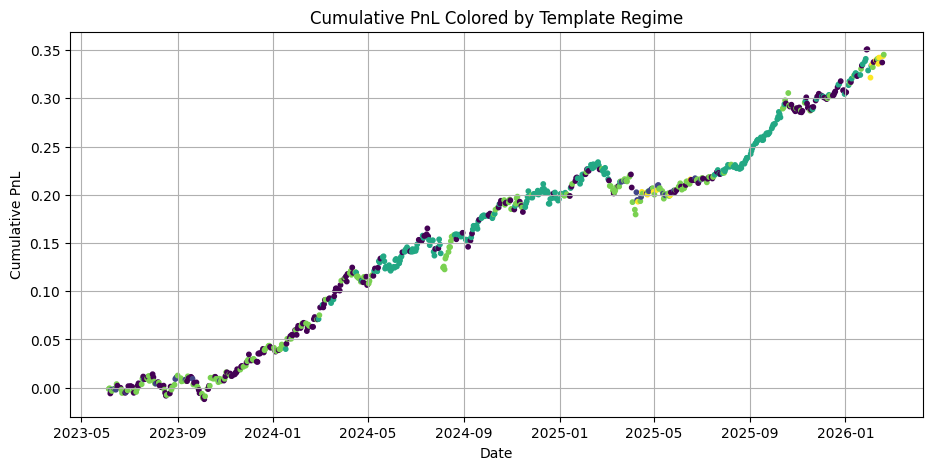
\includegraphics[width=0.95\linewidth]{PRD_pnl.png}
\caption{Cumulative OOS portfolio performance for parametric regime detection.}
\label{fig:prd_pnl}
\end{figure}

\begin{figure}[H]
\centering
\includegraphics[width=0.95\linewidth]{KNN_pnl.png}
\caption{Cumulative OOS portfolio performance for non-parametric KNN.}
\label{fig:knn_pnl}
\end{figure}

\subsection{Rebalancing Dynamics and Turnover}

\begin{table}[H]
\centering
\caption{Rebalancing and Turnover Statistics}
\label{tab:turnover}
\begin{tabular}{lcc}
\toprule
Metric & KNN + MVO & Parametric + MVO \\
\midrule
Average Daily Turnover & 0.5665 & \textbf{0.0081} \\
95\% Turnover Quantile & 1.0000 & \textbf{0.0568} \\
Days with $>1\%$ Turnover & 94.10\% & \textbf{14.35\%} \\
Days with $>5\%$ Turnover & 93.51\% & \textbf{5.62\%} \\
\bottomrule
\end{tabular}
\end{table}

\begin{figure}[H]
\centering
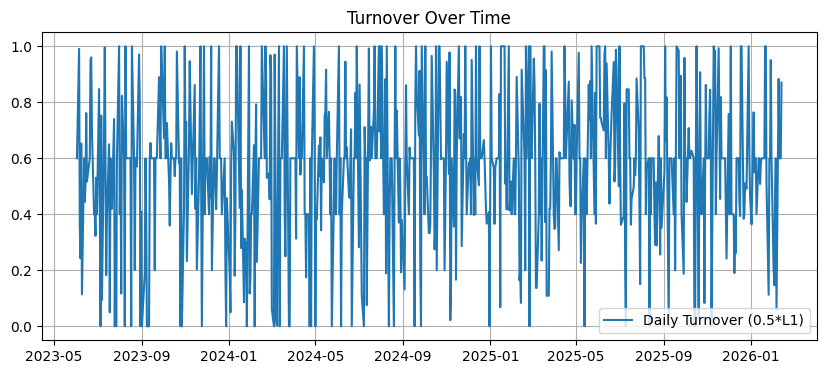
\includegraphics[width=0.95\linewidth]{KNN_rebalancing.png}
\caption{Daily turnover time series for non-parametric KNN + MVO.}
\label{fig:turnover_knn}
\end{figure}
The KNN strategy exhibits persistent high turnover, reflecting instability of nearest-neighbor
sets at daily frequency when used to estimate conditional moments for MVO
\begin{figure}[H]
\centering
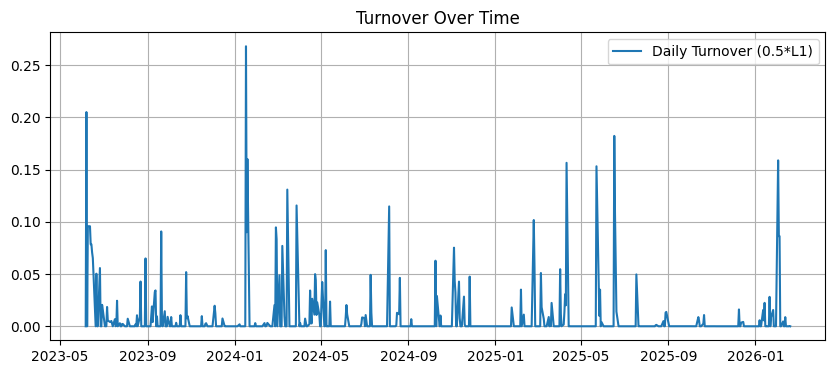
\includegraphics[width=0.95\linewidth]{PRD_rebalancing.png}
\caption{Daily turnover time series for parametric regime detection + MVO.}
\label{fig:turnover_prd}
\end{figure}
Despite daily re-optimization, Parametric Regime Detection produces smoother turnover dynamics due to regime persistence and more stable conditional moment estimates.

\subsection{Average Allocation and Weight Stability}

\begin{table}[H]
\centering
\caption{Average Allocation and Weight Dynamics}
\label{tab:allocation}
\begin{tabular}{lcccc|cccc}
\toprule
& \multicolumn{4}{c}{KNN + MVO} & \multicolumn{4}{c}{Parametric + MVO} \\
\cmidrule(lr){2-5} \cmidrule(lr){6-9}
Asset & Avg Wt & Wt Vol & Time $>10\%$ & Avg $|\Delta w|$
      & Avg Wt & Wt Vol & Time $>10\%$ & Avg $|\Delta w|$ \\
\midrule
SPX  & 0.222430 & 0.252156 & 0.468336 & 0.241619 & 0.216856 & 0.040934 & 0.994092 & 0.003903 \\
BOND & 0.189792 & 0.225578 & 0.459499 & 0.202712 & 0.241904 & 0.108443 & 0.955687 & 0.001764 \\
GOLD & 0.183970 & 0.244556 & 0.403535 & 0.237563 & 0.005020 & 0.014923 & 0.002954 & 0.001878 \\
OIL  & 0.201179 & 0.238252 & 0.456554 & 0.231058 & 0.276775 & 0.054154 & 1.000000 & 0.002500 \\
USD  & 0.202629 & 0.242157 & 0.456554 & 0.220048 & 0.259446 & 0.108841 & 0.940916 & 0.006250 \\
\bottomrule
\end{tabular}
\end{table}

\begin{figure}[H]
\centering
\includegraphics[width=0.98\linewidth]{KNN_weights.png}
\caption{Daily portfolio weights for non-parametric KNN + MVO (stacked area).}
\label{fig:weights_knn}
\end{figure}
The strategy exhibits frequent and large reallocations across all assets, consistent with high turnover.
\begin{figure}[H]
\centering
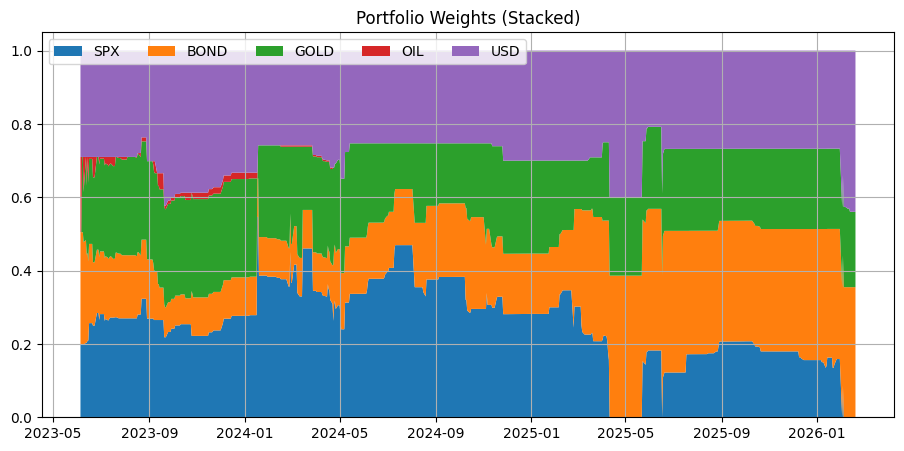
\includegraphics[width=0.98\linewidth]{PRD_weights.png}
\caption{Daily portfolio weights for parametric regime detection + MVO (stacked area).}
\label{fig:weights_prd}
\end{figure}
Allocations are smoother and more persistent for Parametric Regime Detection consistent with lower turnover.

\subsection{Portfolio Concentration}

\begin{table}[H]
\centering
\caption{Portfolio Concentration Metrics}
\label{tab:concentration}
\begin{tabular}{lcc}
\toprule
Metric & KNN + MVO & Parametric + MVO \\
\midrule
Average $N_{\text{eff}}$ & 2.07 & \textbf{3.63} \\
Median $N_{\text{eff}}$  & 1.92 & \textbf{3.70} \\
\bottomrule
\end{tabular}
\end{table}
Parametric regime detection achieves higher effective diversification while trading substantially less, indicating more
stable simultaneous risk exposures
\begin{figure}[H]
\centering
\includegraphics[width=0.95\linewidth]{KNN_concentration.png}
\caption{Effective diversification $N_{\text{eff}}$ for non-parametric KNN + MVO.}
\label{fig:neff_knn}
\end{figure}

\begin{figure}[H]
\centering
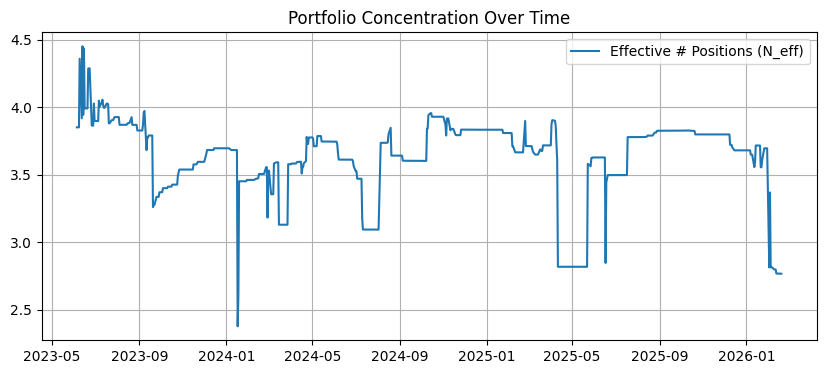
\includegraphics[width=0.95\linewidth]{PRD_concentration.png}
\caption{Effective diversification $N_{\text{eff}}$ for parametric regime detection + MVO.}
\label{fig:neff_prd}
\end{figure}

\subsection{Discussion and Practical Implications}

Non-parametric KNN produces highly unstable conditional moments at daily frequency because nearest-neighbor sets vary substantially across days.
When these moments feed mean--variance optimization, the optimizer reacts aggressively, generating persistent and extreme turnover.
This is reflected in the near-universal rebalancing intensity and higher drawdowns.

Parametric regime detection produces stable, structured conditional moments through predictive model-order selection and template-based identity tracking.
Wasserstein template tracking prevents label permutations and ensures smooth identity evolution without combinatorial matching.
These stability properties propagate into the MVO layer, yielding dramatically lower turnover, stronger drawdown control, and improved risk-adjusted performance.

\section{Economic Interpretation of Template Regimes}
\label{sec:template_regimes}

Because template identities persist over time, we can compute asset and portfolio performance conditional on regime.

\begin{table}[H]
\centering
\caption{Portfolio Performance by Template Regime}
\label{tab:portfolio_by_regime}
\begin{tabular}{lcccccc}
\toprule
Regime & Days & Ann Mean & Ann Vol & Sharpe & Hit Rate & Max DD (within) \\
\midrule
A  & 209 & 0.132748 & 0.052735 & 2.517244 & 0.588517 & -0.039444 \\
B  & 32  & 0.285234 & 0.078569 & 3.630344 & 0.593750 & -0.008506 \\
C  & 212 & 0.148035 & 0.061536 & 2.405666 & 0.627358 & -0.029394 \\
D  & 211 & 0.073687 & 0.057434 & 1.282993 & 0.601896 & -0.039117 \\
E  & 13  & 0.106090 & 0.065074 & 1.630287 & 0.615385 & -0.009055 \\
\bottomrule
\end{tabular}
\end{table}

\begin{table}[H]
\centering
\caption{Asset Performance by Template Regime (Annualized Sharpe)}
\label{tab:asset_sharpe_by_regime}
\begin{tabular}{lccccc}
\toprule
Regime & SPX & BOND & GOLD & OIL & USD \\
\midrule
A  & 2.210756 & 0.995464 & -0.657123 & -0.487256 & 1.933670 \\
B  & 2.245412 & 4.829871 & -1.858978 & -3.483967 & 4.126901 \\
C & 2.398093 & 2.827500 & 0.341027  & -0.331852 & 0.439244 \\
D  & 0.985143 & -2.491856 & 1.630447 & 3.181894  & 0.713300 \\
E  & 1.382953 & 1.469817  & -1.712425 & -0.813208 & -2.906718 \\
\bottomrule
\end{tabular}
\end{table}

\begin{figure}[H]
\centering
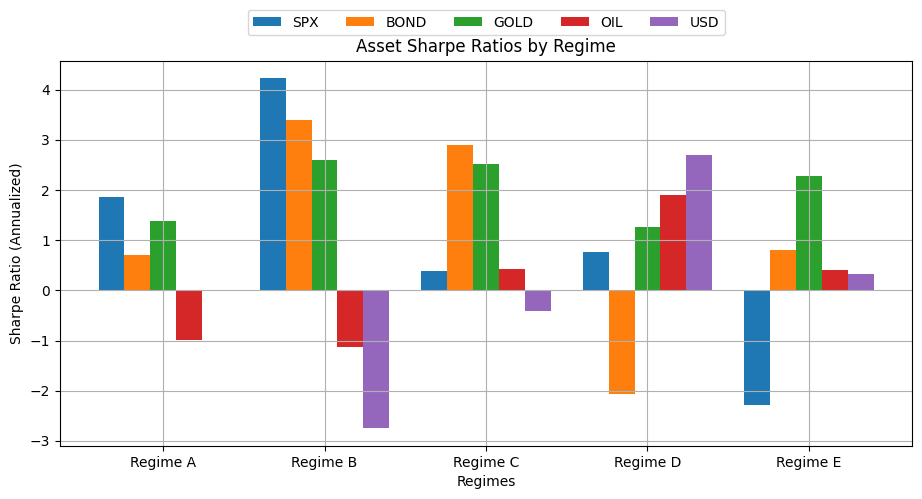
\includegraphics[width=0.95\linewidth]{Regime_sharpes.png}
\caption{Asset Sharpe ratios by regime.}
\label{fig:regime_sharpes}
\end{figure}

\begin{figure}[H]
\centering
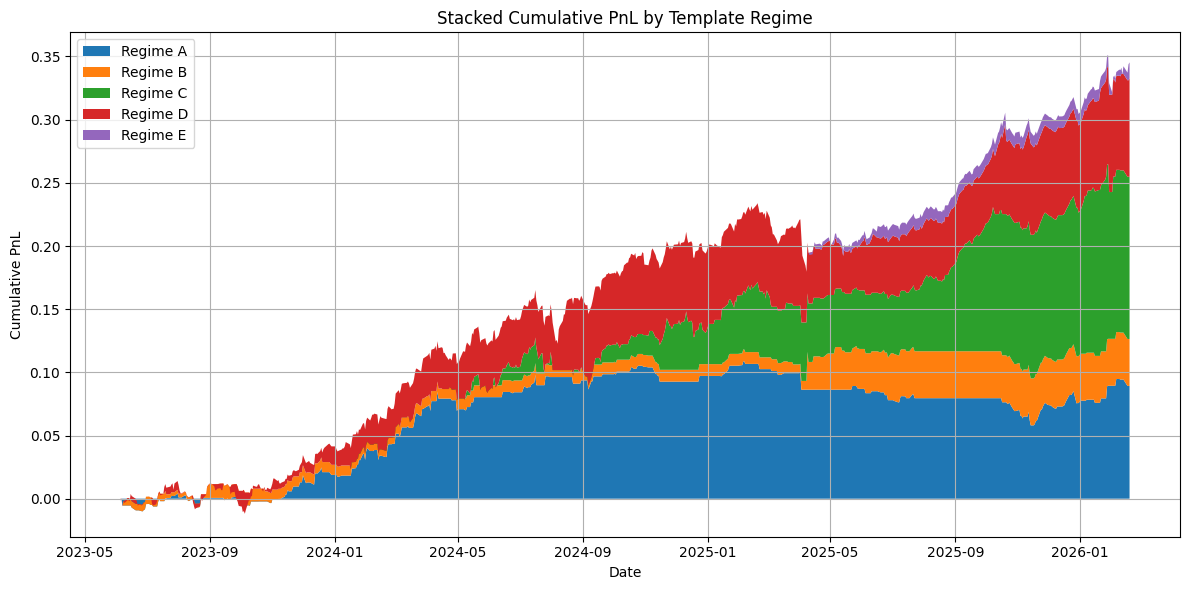
\includegraphics[width=0.95\linewidth]{Pnl_by_regime.png}
\caption{Portfolio performance by regime (templates).}
\label{fig:pnl_by_regime}
\end{figure}

\paragraph{Regime A: Balanced risk-on with defensive USD support.}
Equities and bonds both deliver solid positive Sharpe ratios, while USD also performs well.
This regime resembles a constructive environment with diversified carry and moderate risk-taking.

\paragraph{Regime B: Strong fixed-income and USD regime.}
Bonds and USD exhibit exceptionally high Sharpe ratios, while commodities (gold and oil) are sharply negative.
This pattern is consistent with a pronounced flight-to-quality or disinflationary shock environment.

\paragraph{Regime C: Broad risk-on with equity leadership.}
Equities lead with strong Sharpe and bonds remain positive, while oil is weak and USD is modest.
This resembles a growth-driven expansion with less commodity support.

\paragraph{Regime D: Commodity/real-asset support with weak bonds.}
Oil is strongly positive and gold is supportive, while bonds are negative.
This aligns with reflationary or inflation-linked dynamics where real assets outperform and duration suffers.

\paragraph{Regime E: Short-lived unstable regime.}
This regime appears rarely and exhibits mixed performance: equities and bonds remain positive, but USD is strongly negative and commodities are weak.
Given limited sample size, it is best interpreted cautiously as an episodic transitional regime.
\section{Benchmarking Against Passive Allocations}
\label{sec:benchmarking}

To evaluate whether parametric regime detection delivers economically meaningful improvements beyond passive exposure, we benchmark our strategy against two reference allocations evaluated over the identical strictly out-of-sample (OOS) period:

\begin{itemize}
    \item \textbf{SPX Buy \& Hold:} Passive exposure to the S\&P 500 index.
    \item \textbf{Equal-Weight Portfolio (20\% each):} A static allocation equally distributed across SPX, BOND, GOLD, OIL, and USD.
\end{itemize}

These benchmarks isolate two alternatives:
(i) concentrated equity beta, and
(ii) naive diversification without regime conditioning or optimization.

\subsection{Risk-Adjusted Performance}

Table~\ref{tab:benchmark_sharpe} reports annualized Sharpe and Sortino ratios across strategies.

\begin{table}[H]
\centering
\caption{Risk-Adjusted Performance (Out-of-Sample)}
\label{tab:benchmark_sharpe}
\begin{tabular}{lcc}
\toprule
Strategy & Sharpe & Sortino \\
\midrule
Parametric Regime Detection (HMM + MVO) & \textbf{2.16} & \textbf{2.79} \\
Equal-Weight (20\%) & 1.54 & 2.19 \\
SPX Buy \& Hold & 1.83 & 2.20 \\
\bottomrule
\end{tabular}
\end{table}

The regime-aware strategy achieves the highest Sharpe and Sortino ratios. Relative to SPX Buy \& Hold, the Sharpe ratio improves from 1.83 to 2.16, while the Sortino ratio increases materially from 2.20 to 2.79, indicating superior downside risk management. Compared to the equal-weight portfolio, the improvement is even more pronounced, highlighting the value of conditional covariance modeling and state-dependent allocation.

\subsection{Cumulative Performance Comparison}

Figure~\ref{fig:cum_benchmark} presents cumulative log returns for all three strategies over the OOS period.

\begin{figure}[H]
\centering
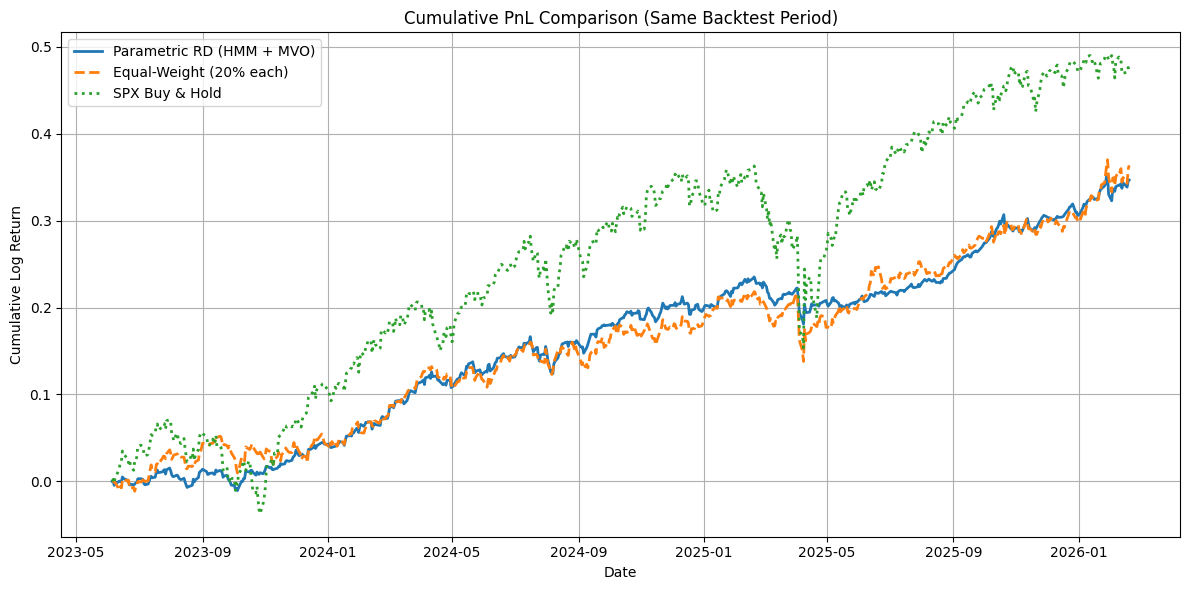
\includegraphics[width=0.95\linewidth]{benchmark_cum_pnl.png}
\caption{Cumulative out-of-sample log returns: Parametric Regime Detection vs Equal-Weight vs SPX Buy \& Hold.}
\label{fig:cum_benchmark}
\end{figure}


The cumulative performance profile illustrates three distinct dynamics:

\begin{enumerate}
    \item \textbf{SPX Buy \& Hold} captures strong equity rallies but exhibits higher volatility and deeper interim drawdowns.
    
    \item \textbf{Equal-Weight} smooths concentration risk but lacks conditional responsiveness to evolving cross-asset covariance structures.
    
    \item \textbf{Parametric Regime Detection} compounds more steadily, balancing participation in favorable regimes with risk reduction during adverse states.
\end{enumerate}

\subsection{Economic Interpretation}

The improvement in risk-adjusted performance reflects structural advantages of regime-aware allocation:

\begin{itemize}
    \item \textbf{State-Conditional Risk Control:} Portfolio weights adapt to changes in the joint return distribution rather than relying on unconditional averages.
    \item \textbf{Downside Mitigation:} Higher Sortino ratios indicate more efficient drawdown containment.
    \item \textbf{Volatility Drag Reduction:} Smoother compounding improves long-term growth efficiency.
\end{itemize}

Overall, the benchmarking results demonstrate that parametric regime detection adds value beyond both passive equity exposure and static diversification. The gains are especially pronounced in downside-adjusted performance, reinforcing the importance of structured regime inference in daily portfolio construction.
\section{Conclusion}

We study explainable, regime-aware portfolio construction at daily frequency and show that the regime inference mechanism is a first-order driver
of realized turnover, drawdowns, and risk-adjusted performance.
A non-parametric KNN approach can induce unstable conditional moments at daily frequency, leading to persistent and extreme trading intensity.
In contrast, parametric regime detection based on a predictive-selected Gaussian HMM and Wasserstein template tracking produces stable regime identity,
smooths conditional moments, and yields markedly improved implementation characteristics.

Empirically, parametric regime detection delivers higher OOS Sharpe (2.15 vs.\ 1.80), substantially lower maximum drawdown (-5.35\% vs.\ -12.52\%),
and orders-of-magnitude lower turnover (0.008 average daily vs.\ 0.567), while also improving effective diversification ($N_{\text{eff}}$).
Because templates preserve regime identity through time, the resulting regimes admit clear economic narratives and enable performance attribution by regime.

\begin{thebibliography}{99}

\bibitem{Hamilton1989}
Hamilton, J. D. (1989).
\newblock A New Approach to the Economic Analysis of Nonstationary Time Series and the Business Cycle.
\newblock \emph{Econometrica}, 57(2), 357--384.

\bibitem{AngBekaert2002}
Ang, A., and Bekaert, G. (2002).
\newblock International Asset Allocation with Regime Shifts.
\newblock \emph{Review of Financial Studies}, 15(4), 1137--1187.

\bibitem{AngBekaert2004}
Ang, A., and Bekaert, G. (2004).
\newblock How Do Regimes Affect Asset Allocation?
\newblock \emph{Financial Analysts Journal}, 60(2), 86--99.

\bibitem{GuidolinTimmermann2007}
Guidolin, M., and Timmermann, A. (2007).
\newblock Asset Allocation under Multivariate Regime Switching.
\newblock \emph{Journal of Economic Dynamics and Control}, 31(11), 3503--3544.

\bibitem{GuidolinTimmermann2008}
Guidolin, M., and Timmermann, A. (2008).
\newblock International Asset Allocation under Regime Switching, Skew, and Kurtosis Preferences.
\newblock \emph{Review of Financial Studies}, 21(2), 889--935.

\bibitem{DeMiguel2009}
DeMiguel, V., Garlappi, L., and Uppal, R. (2009).
\newblock Optimal Versus Naive Diversification: How Inefficient is the 1/N Portfolio Strategy?
\newblock \emph{Review of Financial Studies}, 22(5), 1915--1953.

\bibitem{LedoitWolf2004}
Ledoit, O., and Wolf, M. (2004).
\newblock A Well-Conditioned Estimator for Large-Dimensional Covariance Matrices.
\newblock \emph{Journal of Multivariate Analysis}, 88(2), 365--411.
\bibitem{Hirsa2024}
Hirsa, A., Xu, S., and Malhotra, S. (2024).
\newblock Robust Rolling Regime Detection (R2-RD): A Data-Driven Perspective of Financial Markets.
\newblock SSRN Working Paper.
\end{thebibliography}

\end{document}